\documentclass[11pt,a4paper]{article}
\usepackage[margin=2.2cm]{geometry}
\usepackage{graphicx,booktabs,url,amsmath}
\usepackage[hidelinks]{hyperref}
\usepackage{placeins}
\usepackage{float}
\graphicspath{{../../../fullsim_analysis/results/bench/2026-10-23/}}
\title{Bench data of 23 October 2026: green and red adapter boards}
\author{JJ}
\date{23 October 2026}
\begin{document}
\maketitle

On 23 October Laura Navarro repeated menu 1 (Citiroc noise) with boards 0 and 1, connected to
the SiPM matrices through the CAEN ``red'' adapter boards instead of our ``green'' ones, and
with the FPGA of board 1 upgraded. This report compares the noise of the two boards with the
two adapters. The method of the noise analysis is that of the report of 22 October.

\section{Data}

The data are nine pedestal runs (Table~\ref{tab:runs}), taken with the SiPMs biased at 36.5~V,
below breakdown, and a periodic trigger every 1~ms. Each run has about 10\,000 events per
board. Both boards run firmware 0xa7070800, which makes channels 0--31 of board 1 readable
(F7). The low gain is shaped at 87.5~ns in all runs, and the detector was at 21--22~$^\circ$C.

\begin{table}[H]
\centering
\small
\begin{tabular}{llll}
\toprule
Runs & Purpose & HG shaping & HoldDelay \\
\midrule
42, 43, 44 & noise against shaping & 25, 50, 87.5 ns & 0 ns \\
45--49 & pedestal against HoldDelay & 25 ns & 96, 200, 296, 400, 496 ns \\
50 & stability (repeats run 42) & 25 ns & 0 ns \\
\bottomrule
\end{tabular}
\caption{Pedestal runs of 23 October, boards 0 and 1, red adapter boards.}
\label{tab:runs}
\end{table}

\begin{figure}[H]
\centering
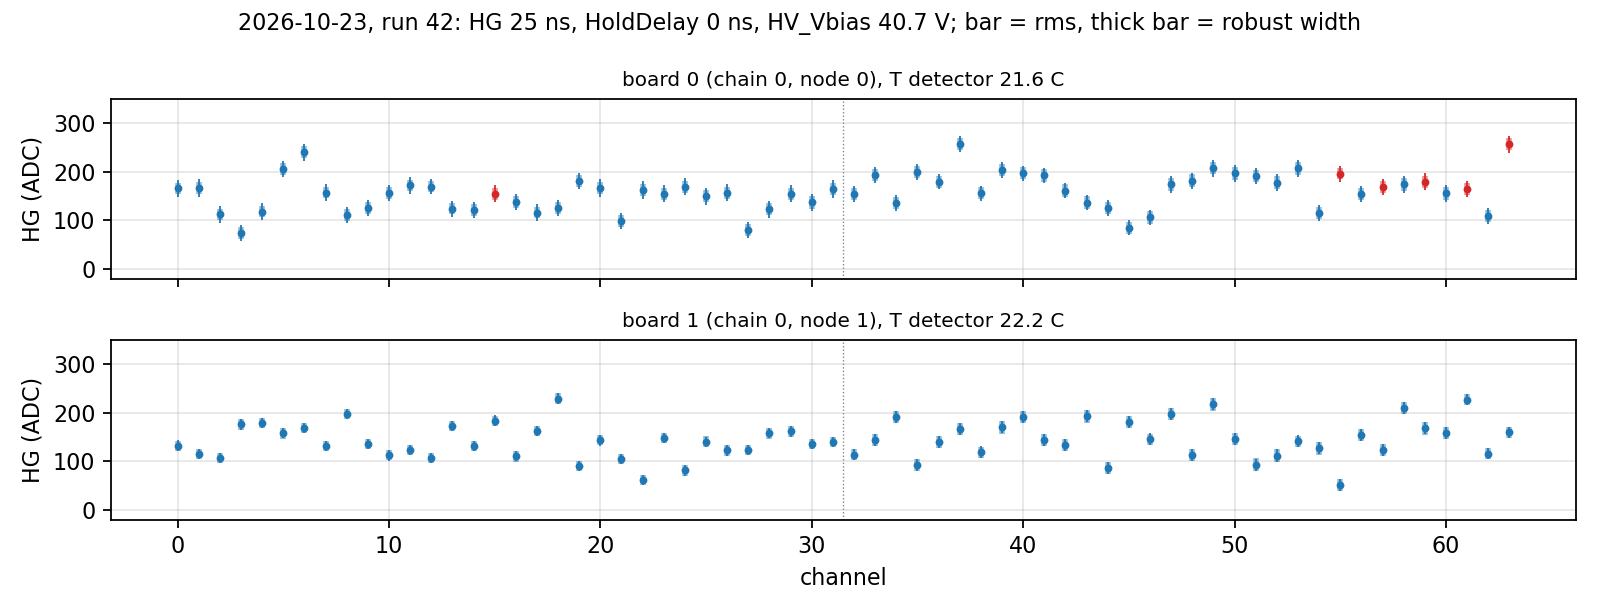
\includegraphics[width=0.92\textwidth]{bench_pedestals.png}
\caption{Run 42 (HG 25~ns, HoldDelay 0): mean of the high gain against the channel for boards 0
and 1, with the rms as error bar and the robust width (interquartile range / 1.349) as a
thicker bar.}
\label{fig:ped}
\end{figure}

Figure~\ref{fig:ped} shows the pedestal of every channel of the two boards in run 42, with its
rms as error bar. The pedestals vary from channel to channel between 52 and 257 ADC counts, and
all 128 channels are read.

\section{Noise}

\begin{table}[H]
\centering
\small
\begin{tabular}{llcccccc}
\toprule
board & channels & adapter & run & $\sigma_\mathrm{tot}$ & $\sigma_\mathrm{coh}$ & $\sigma_\mathrm{inc}$ & $\sigma_\mathrm{coh}^2/\sigma_\mathrm{tot}^2$ \\
\midrule
0 & 0--31 & green & 26 & 12.0 & 6.0 & 10.4 & 0.25 \\
0 & 0--31 & red & 42 & 12.1 & 6.0 & 10.4 & 0.25 \\
0 & 32--63 & green & 26 & 12.3 & 7.0 & 10.2 & 0.32 \\
0 & 32--63 & red & 42 & 12.5 & 7.2 & 10.2 & 0.33 \\
1 & 0--31 & green & -- & \multicolumn{4}{c}{not read (F7)} \\
1 & 0--31 & red & 42 & 10.7 & 5.5 & 9.1 & 0.26 \\
1 & 32--63 & green & 26 & 12.3 & 6.4 & 10.5 & 0.27 \\
1 & 32--63 & red & 42 & 12.3 & 6.5 & 10.5 & 0.28 \\
\bottomrule
\end{tabular}

\caption{Total, coherent and incoherent noise of the high gain (ADC counts) and fraction of the
variance that is coherent, for each chip of boards 0 and 1, at 25~ns and HoldDelay 0, with the
green adapters (run 26, 22 October) and the red ones (run 42).}
\label{tab:comp}
\end{table}

At 25~ns the noise of every chip is the same with the two adapters, within 0.2 counts in each
component (Table~\ref{tab:comp}). The coherent noise, a quarter to a third of the variance,
does not come from our adapter boards. Channels 0--31 of board 1, read for the first time, are
somewhat quieter than the other three chips: 10.7 counts in total, with 5.5 coherent.

\begin{figure}[H]
\centering
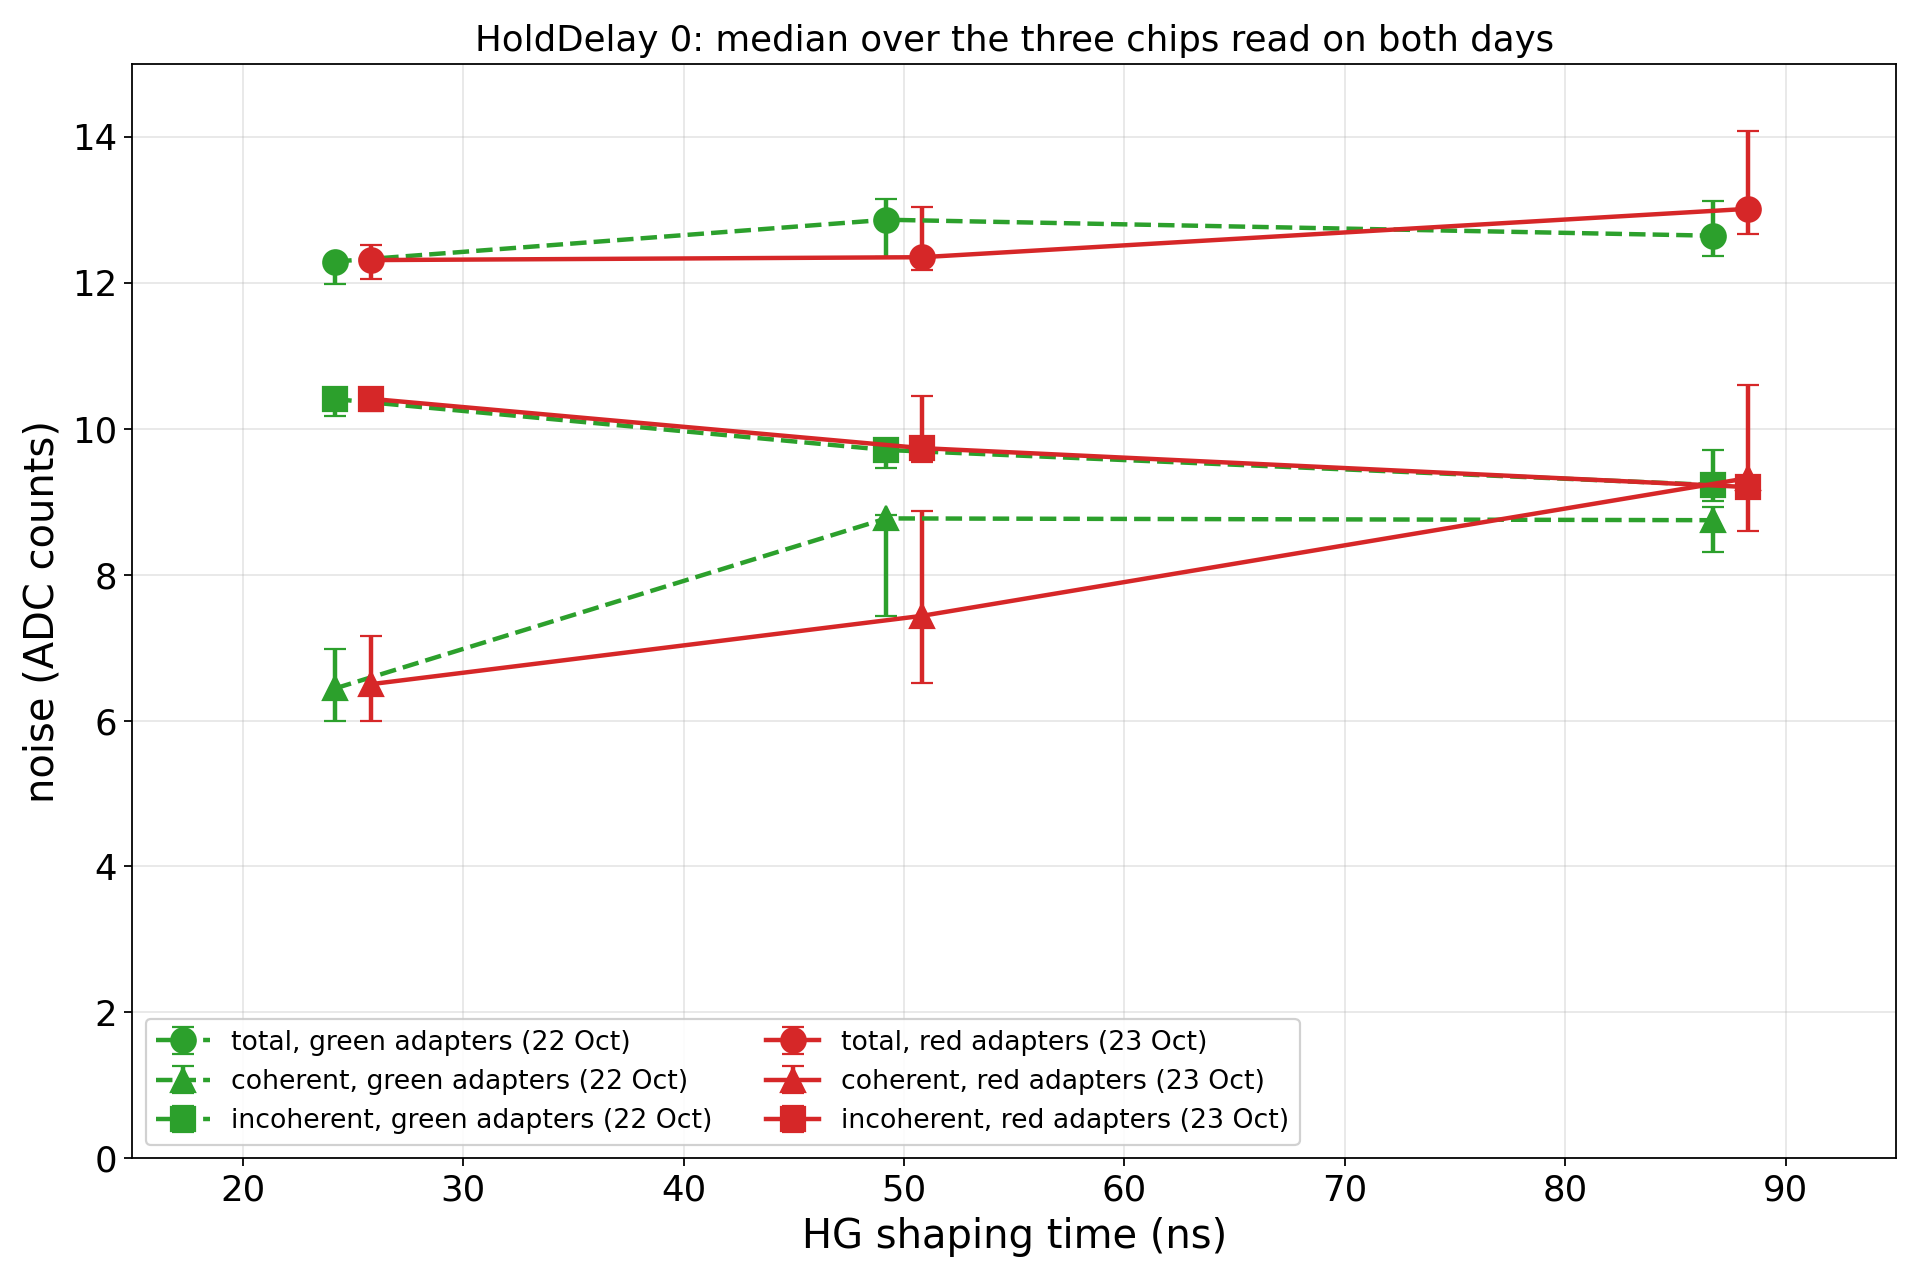
\includegraphics[width=0.8\textwidth]{compare_shaping.png}
\caption{Total, coherent and incoherent noise of the high gain against the shaping time,
HoldDelay 0, median over the three chips read on both days (both chips of board 0, channels
32--63 of board 1), bars from the lowest to the highest chip: green adapters (22 October,
dashed) and red adapters (23 October, solid).}
\label{fig:shaping}
\end{figure}

Against the shaping time (Figure~\ref{fig:shaping}) the total and incoherent noise are the same
on both days, and the incoherent noise falls with a longer shaping as on 22 October. The
coherent noise of board 0 is also the same, chip by chip, at every shaping. Board 1, channels
32--63, behaves differently: with the red adapter its coherent noise stays at 6.5 counts at 25
and 50~ns and jumps to 10.6 at 87.5~ns, where on 22 October it was 6.4, 8.8 and 8.7. Its
newly read channels 0--31 show a coherent noise that does not depend on the shaping (5.5--5.6
counts). The shaping applied to both chips, read from the configuration stored in the files,
is the one requested.

\begin{figure}[H]
\centering
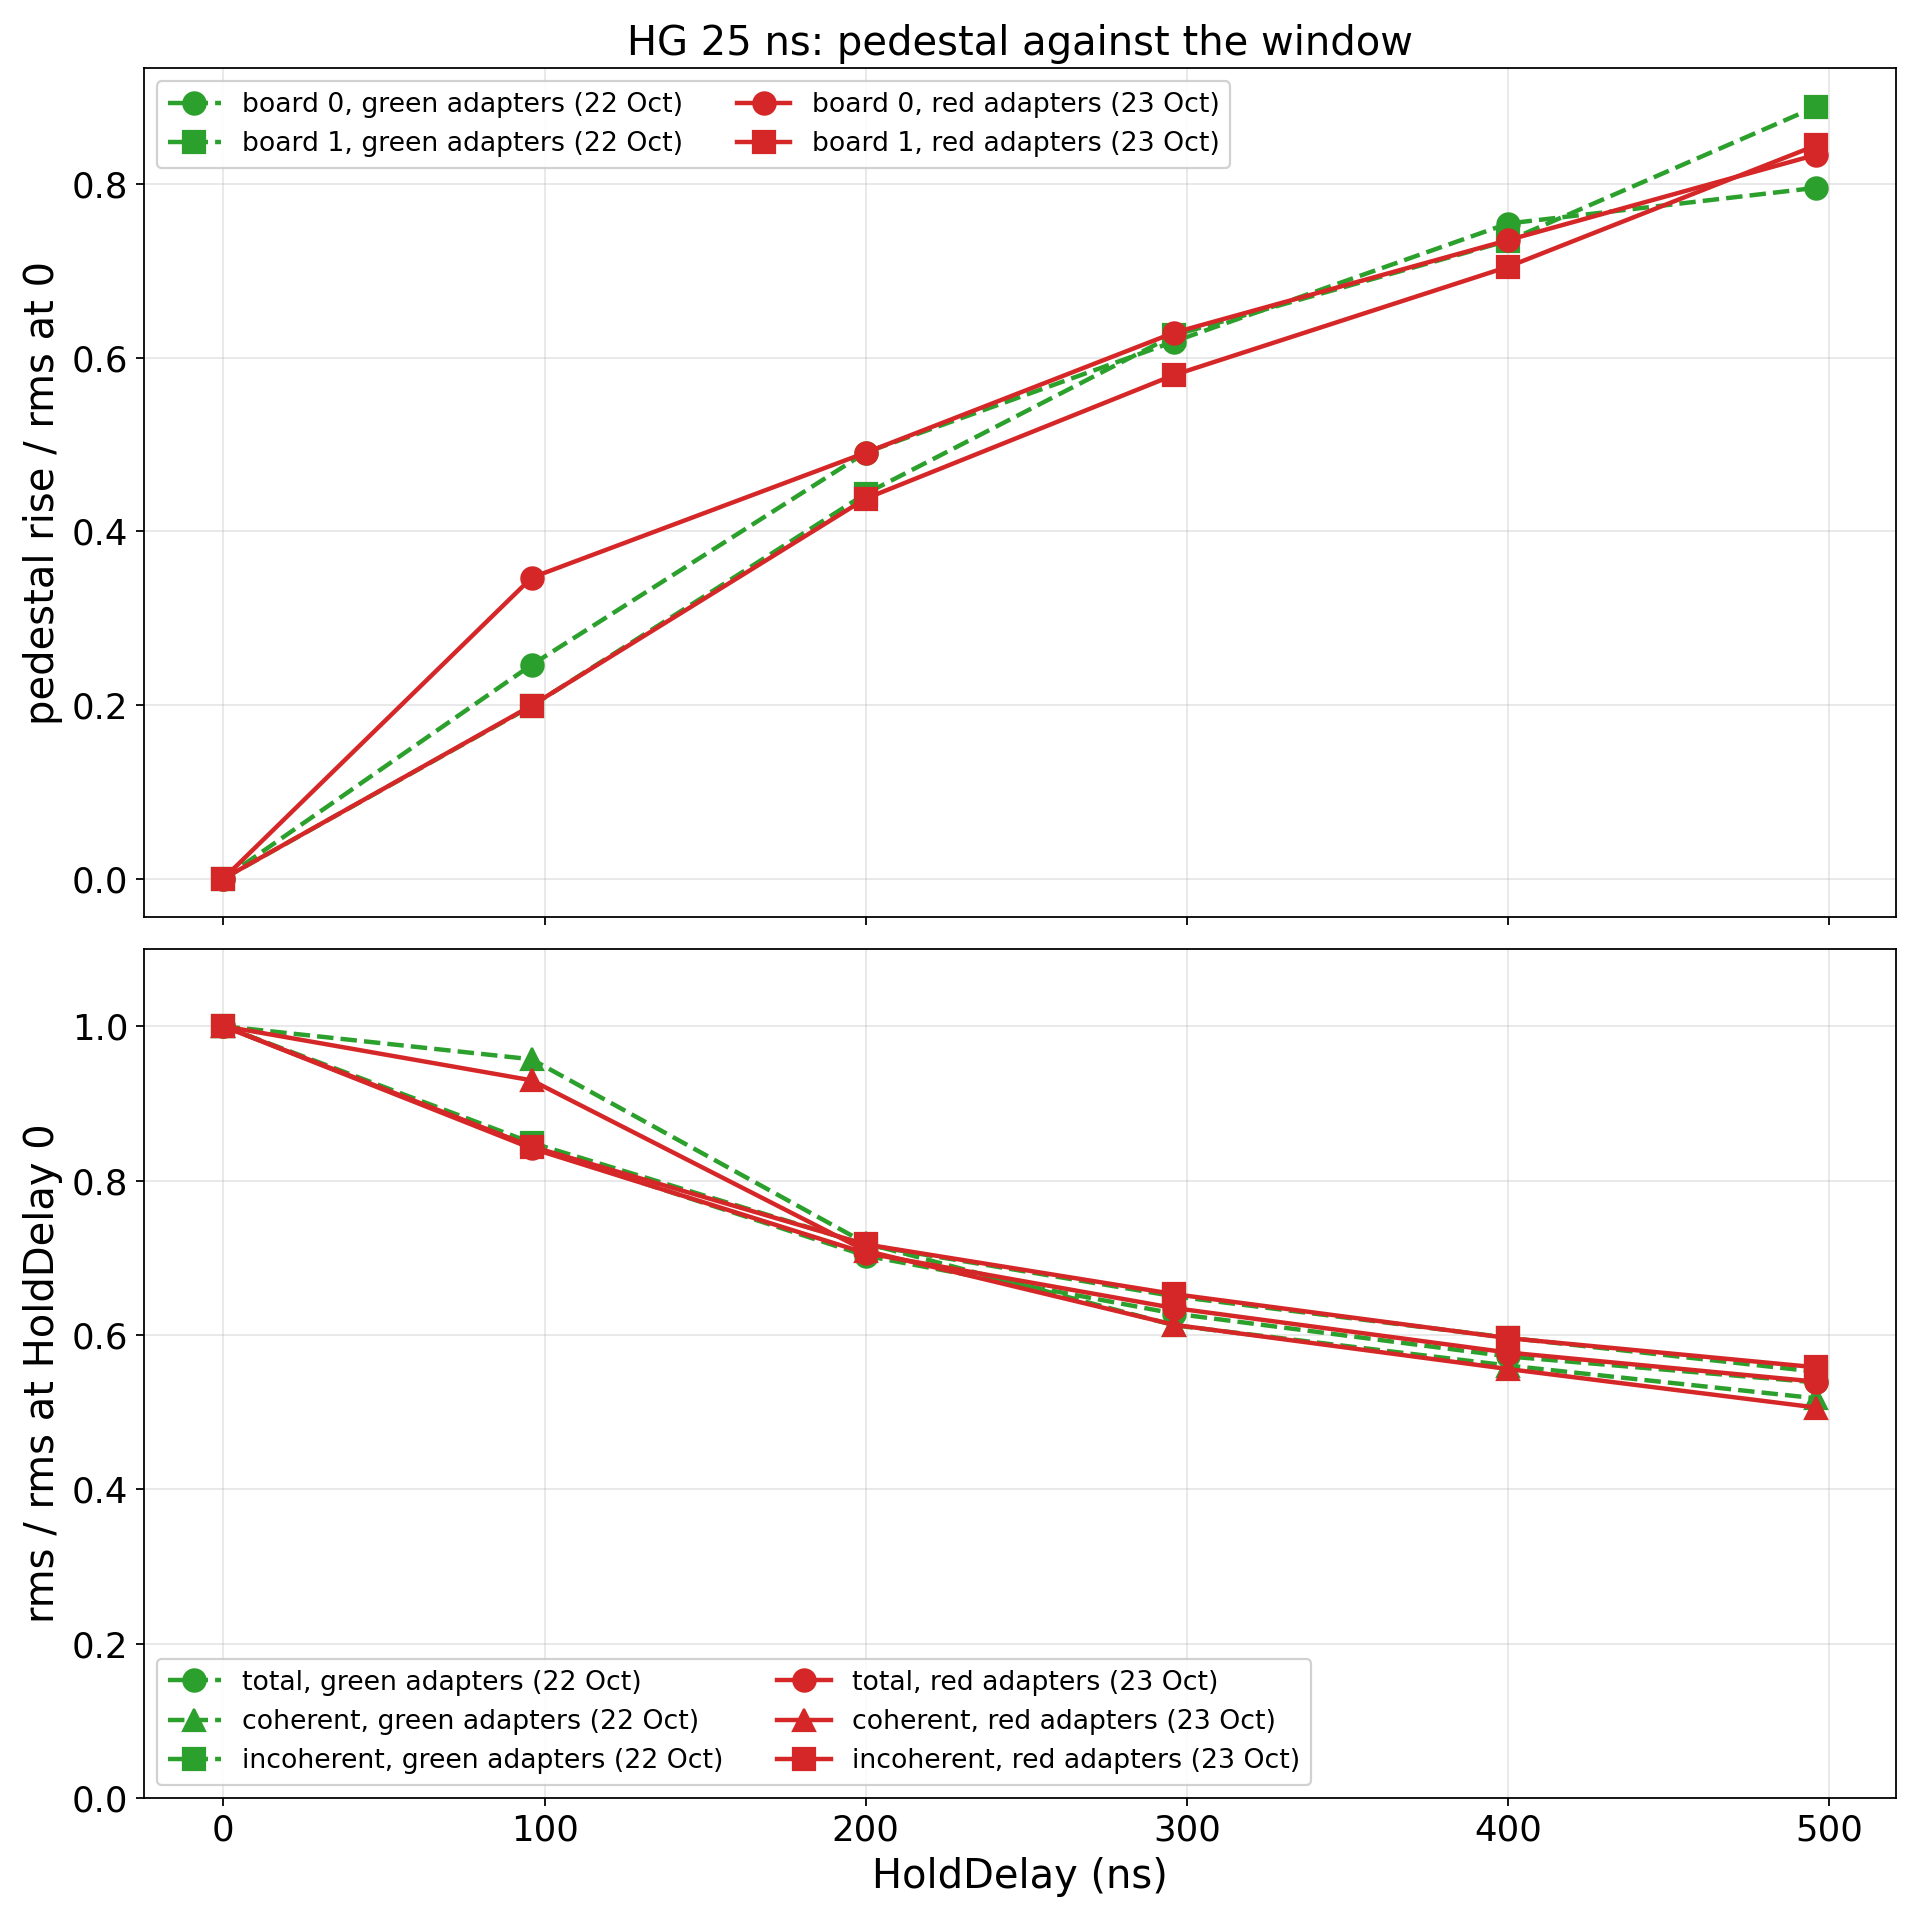
\includegraphics[width=0.8\textwidth]{compare_holddelay.png}
\caption{High gain at 25~ns against HoldDelay, green adapters (dashed) and red adapters
(solid): rise of the pedestal in units of its rms at HoldDelay 0, median over the channels of
each board (top), and total, coherent and incoherent rms relative to HoldDelay 0, median over
the three chips read on both days (bottom).}
\label{fig:hold}
\end{figure}

With a longer HoldDelay the pedestal rises and narrows in the same way with both adapters
(Figure~\ref{fig:hold}).

The common modes of the two chips of board 0 are correlated by 0.65, 0.76 and 0.75 at 25, 50
and 87.5~ns (0.66, 0.77 and 0.81 on 22 October), those of the two chips of board 1 by 0.57,
0.57 and 0.28, and chips of different boards by less than 0.1: the common mode is still a
per-board effect.

The common-mode jumps of board 0 (F10) persist with the red adapter: 21 to 61 per chip in
runs 42--45, on both chips, and none in runs 46--50. Board 1 has none. They do not come from our
adapter board.

\section{Blind channels}

\begin{figure}[H]
\centering
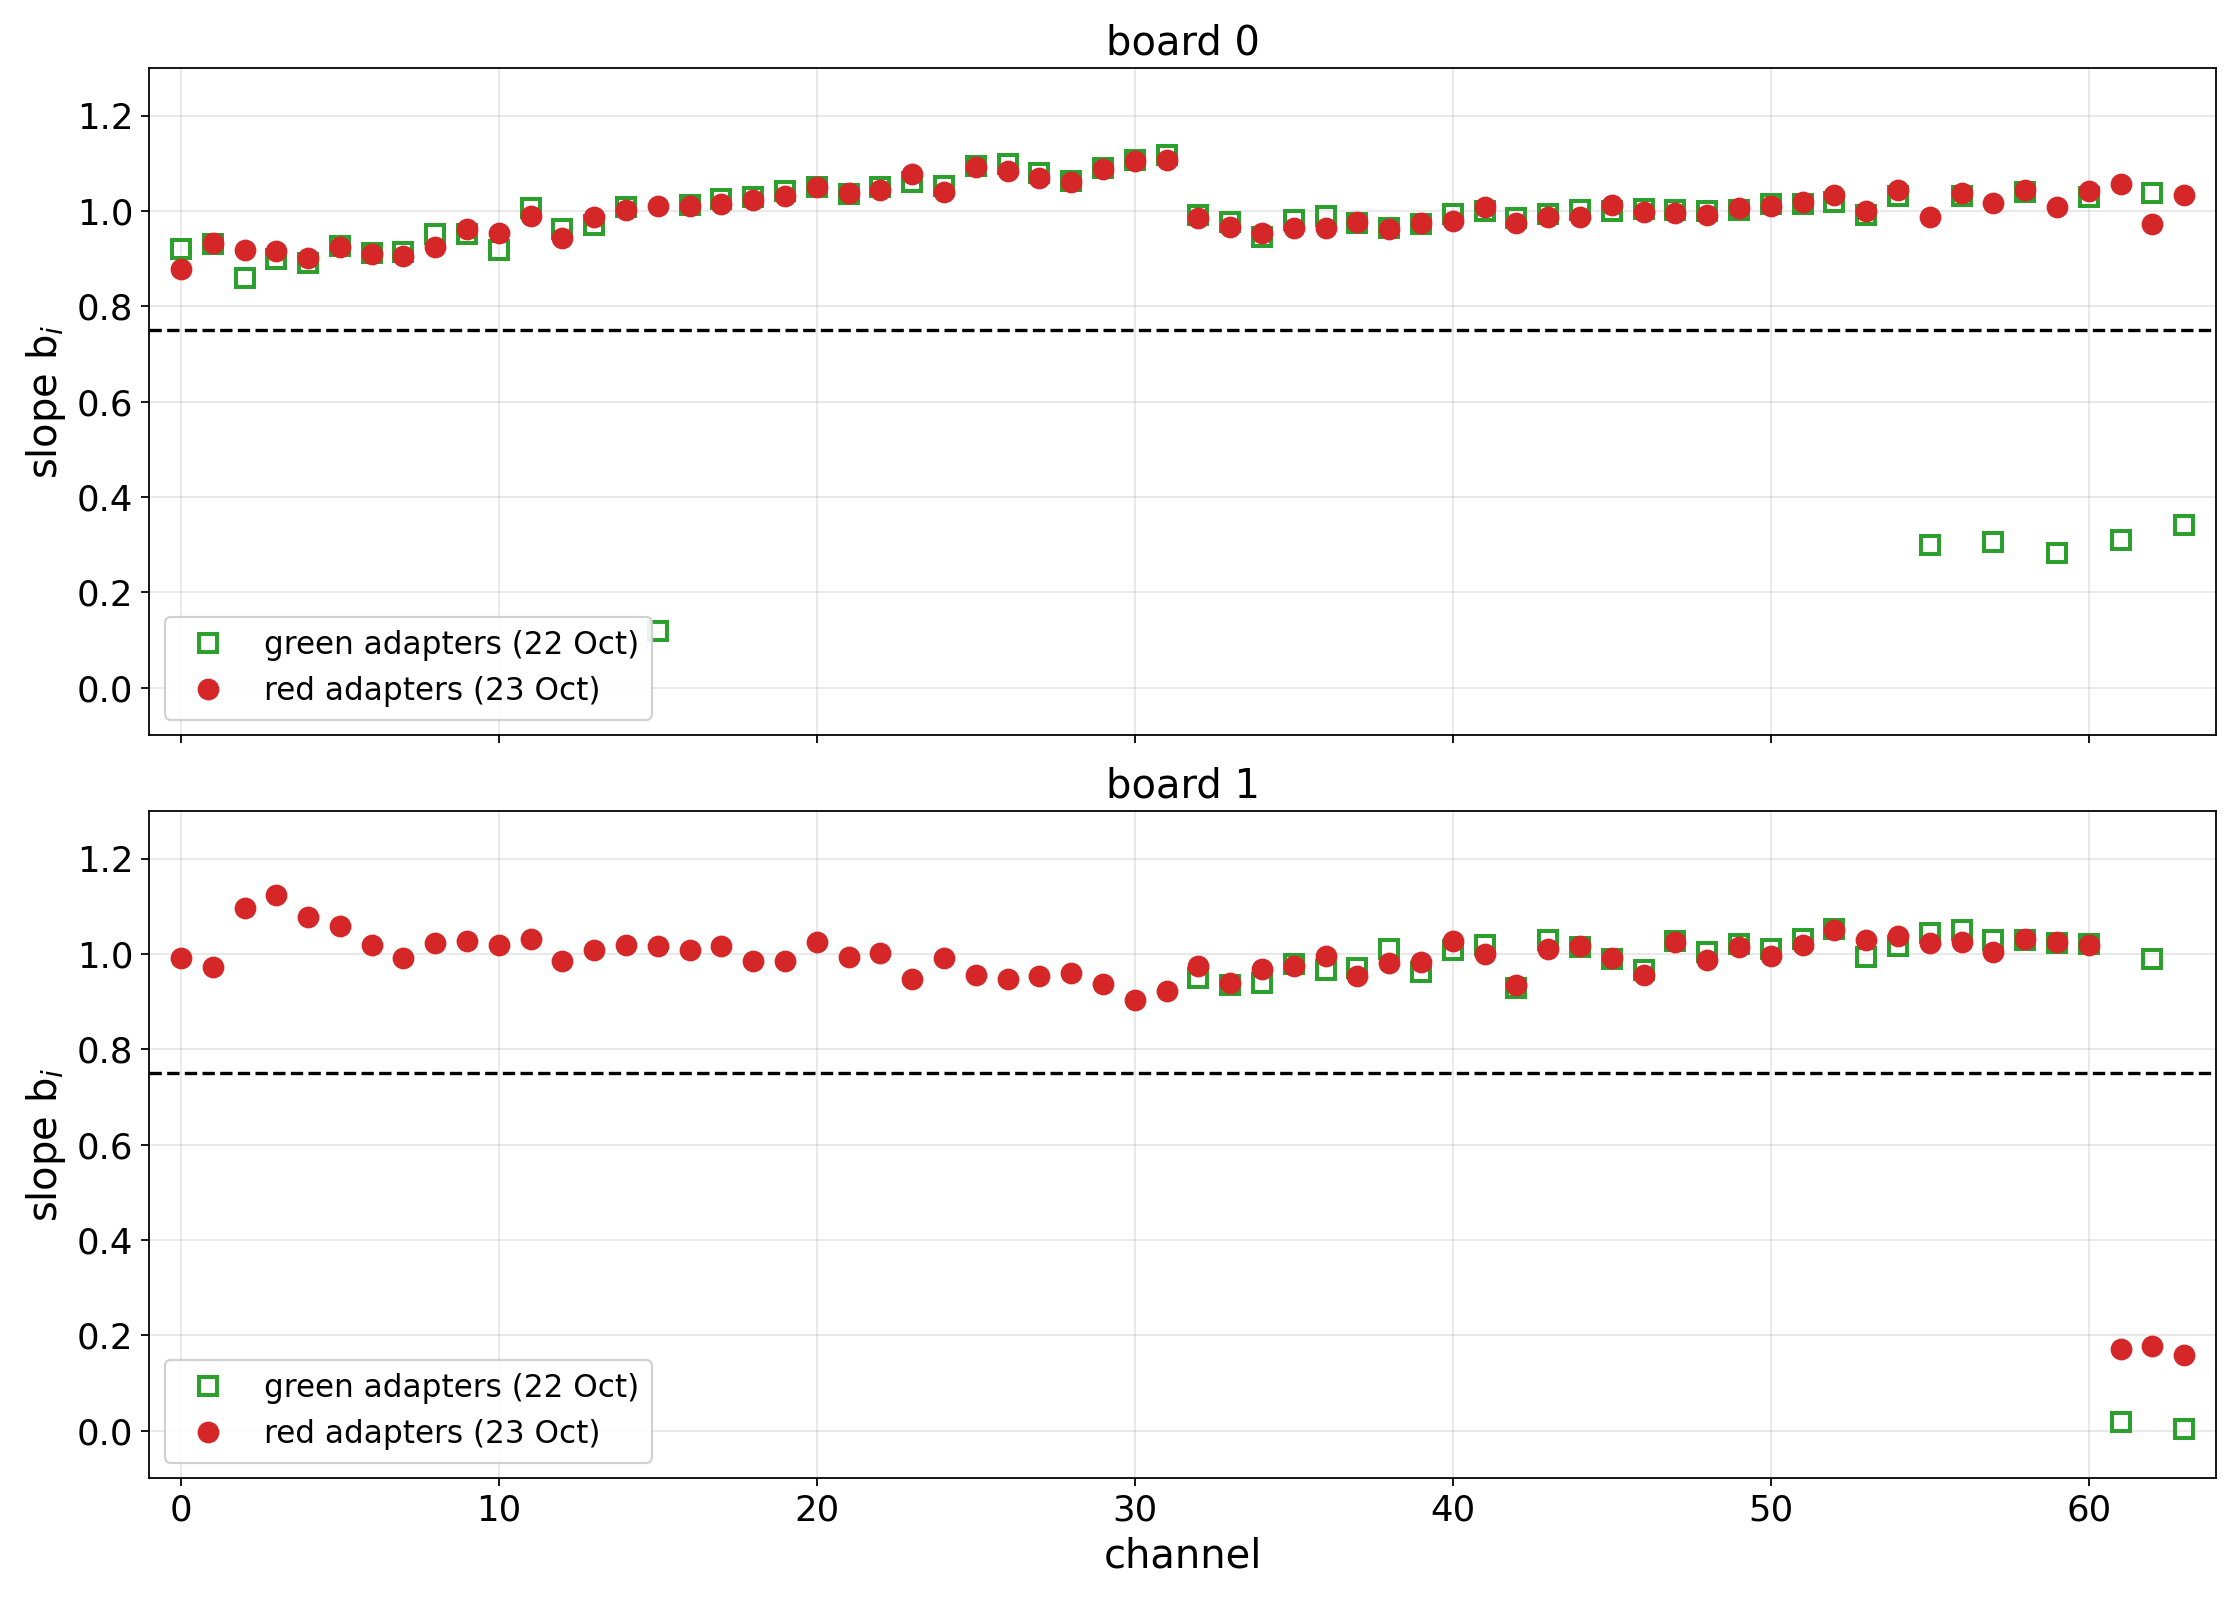
\includegraphics[width=\textwidth]{compare_slopes.png}
\caption{Slope of each channel against the common mode of its chip, median over the runs with
HoldDelay 0, for boards 0 and 1: green adapters (open squares, 22 October) and red adapters
(full circles, 23 October). Below the dashed line (0.75) the channels are blind.}
\label{fig:slopes}
\end{figure}

Figure~\ref{fig:slopes} shows the slope of every channel against the common mode of its chip on
both days. With the green adapter board 0 had six blind channels (15, 55, 57, 59, 61 and 63);
with the red one it has none: those channels were lost in our adapter board. Board 1 had
channels 61 and 63 blind with the green adapter, and with the red one 61, 62 and 63 are blind
(slopes 0.16--0.18, against 0.88 or more for every other channel): there the fault is not in
the adapter but in the SiPM matrix, the cable or the connector on the board side. With the red
adapters no channel is dead in the four chips.

\begin{table}[H]
\centering
\small
\begin{tabular}{llll}
\toprule
Chip & Channels & Green adapter (22 October) & Red adapter (23 October) \\
\midrule
board 0, chip 0 & 0--31 & 15 & none \\
board 0, chip 1 & 32--63 & 55, 57, 59, 61, 63 & none \\
board 1, chip 0 & 0--31 & not read (F7) & none \\
board 1, chip 1 & 32--63 & 61, 63 & 61, 62, 63 \\
\bottomrule
\end{tabular}
\caption{Blind channels of each chip of boards 0 and 1 with the two adapter boards.}
\label{tab:blind}
\end{table}

\section{Issues}

\begin{itemize}
\item \textbf{Blind channels of board 1 (F4).} Channels 61--63 of board 1 stay blind with the
  red adapter. Boards 3 and 4, which had blind channels with the green adapters (45, 47, 49 and
  60; 59, 61 and 63), have not been measured with the red ones; board 4 needs the FPGA upgrade
  first (F7).
\item \textbf{Common-mode jumps of board 0 (F10)}, unchanged with the red adapter.
\item \textbf{Coherent noise of board 1.} With the red adapter and the new firmware it no longer
  follows the shaping as on 22 October: flat in channels 0--31, flat up to 50~ns and higher at
  87.5~ns in channels 32--63. The configuration applied is the one requested.
\end{itemize}

\end{document}
